\section{Evaluation}
%TODO: Is there a good technical reason why every \absmachine machine
% should have exactly one large stateful atom as opposed to many small stateful atoms?
% TODO: Show how pipeline width / depth changes
% by adding more complicated atoms? This might be a little more work though.
\label{s:eval}

\begin{table}[!t]
  \begin{scriptsize}
  \begin{tabular}{|p{0.1\textwidth}|p{0.35\textwidth}|}
    \hline
    Atom & Description \\
    \hline
    Write & Write packet field/constant into single state variable. \\
    \hline
    ReadAddWrite (RAW) & Add packet field/constant to state variable (OR) Write packet field/constant into state variable. \\
    \hline
    Predicated ReadAddWrite (RAW) & Execute RAW on state variable only if a predicate is true, else leave unchanged. \\
    \hline
    IfElse ReadAddWrite (IfElseRaw) & Execute two separate RAWs: one each for when a predicate is true or false.\\
    \hline
    Subtract (Sub) & Same as IfElseRaw, but also allow subtracting a packet field/constant. \\
    \hline
    Nested Ifs (Nested) & Same as Sub, but with an additional level of nesting that provides 4-way predication. \\
    \hline
    Paired updates (pairs) & Same as Nested, but allow updates to a pair of state variables, where predicates can use both state variables. \\
    \hline
  \end{tabular}
  \end{scriptsize}
  \caption{Atoms used in evaluation. Appendix A provides the SKETCH code and
  circuit diagrams for these atoms.}
  \label{tab:templates}
\end{table}

\begin{table}[!t]
  \begin{scriptsize}
    \begin{tabular}{|p{0.08\textwidth}|p{0.3\textwidth}|p{0.03\textwidth}|}
  \hline
  Atom & Circuit & Circuit depth \\
  \hline
  Write & 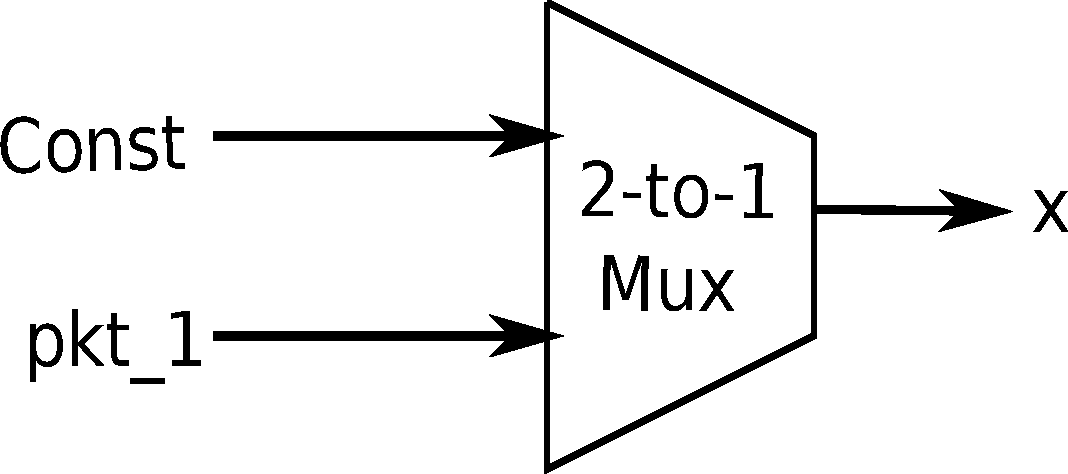
\includegraphics[width=0.2\textwidth]{rw.pdf} & 1 \\
  \hline
  ReadAddWrite (RAW) & 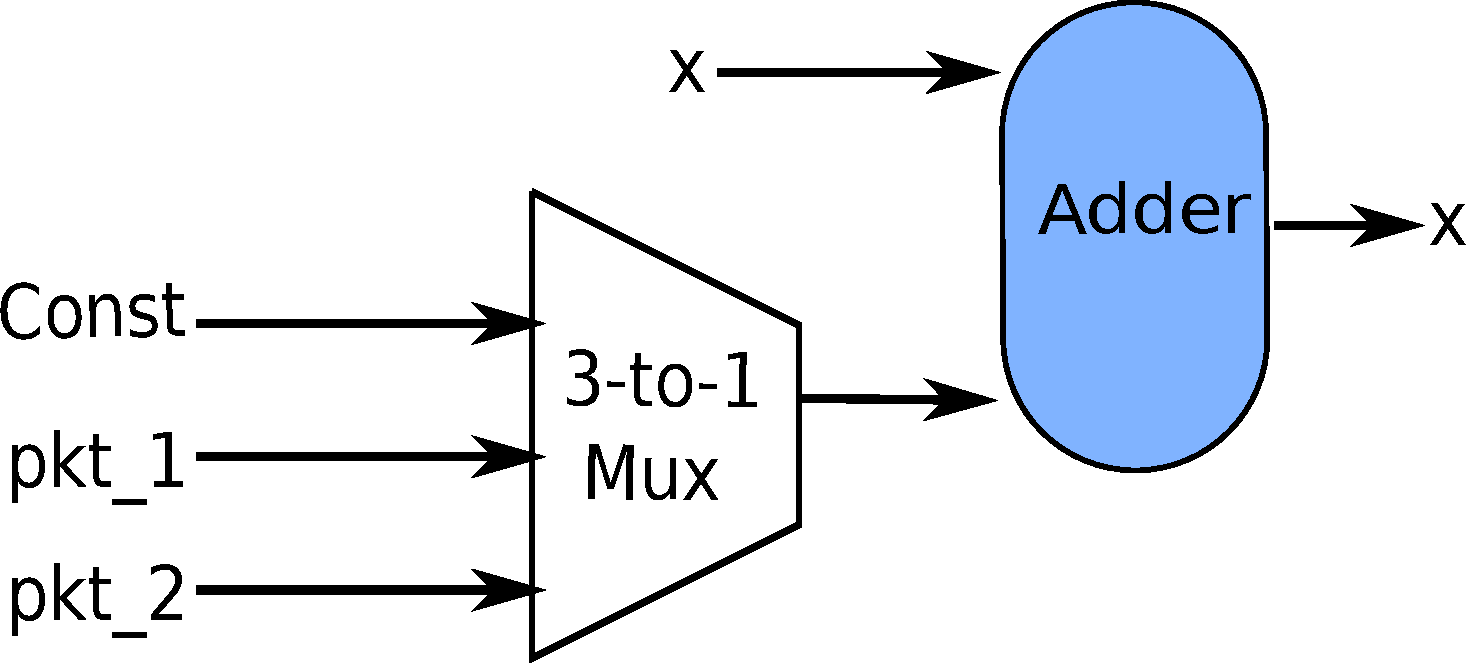
\includegraphics[width=0.2\textwidth]{raw.pdf} & 2\\
  \hline
  \pbox{0.1\textwidth}
  {Predicated\\
  ReadAddWrite (PRAW)} & 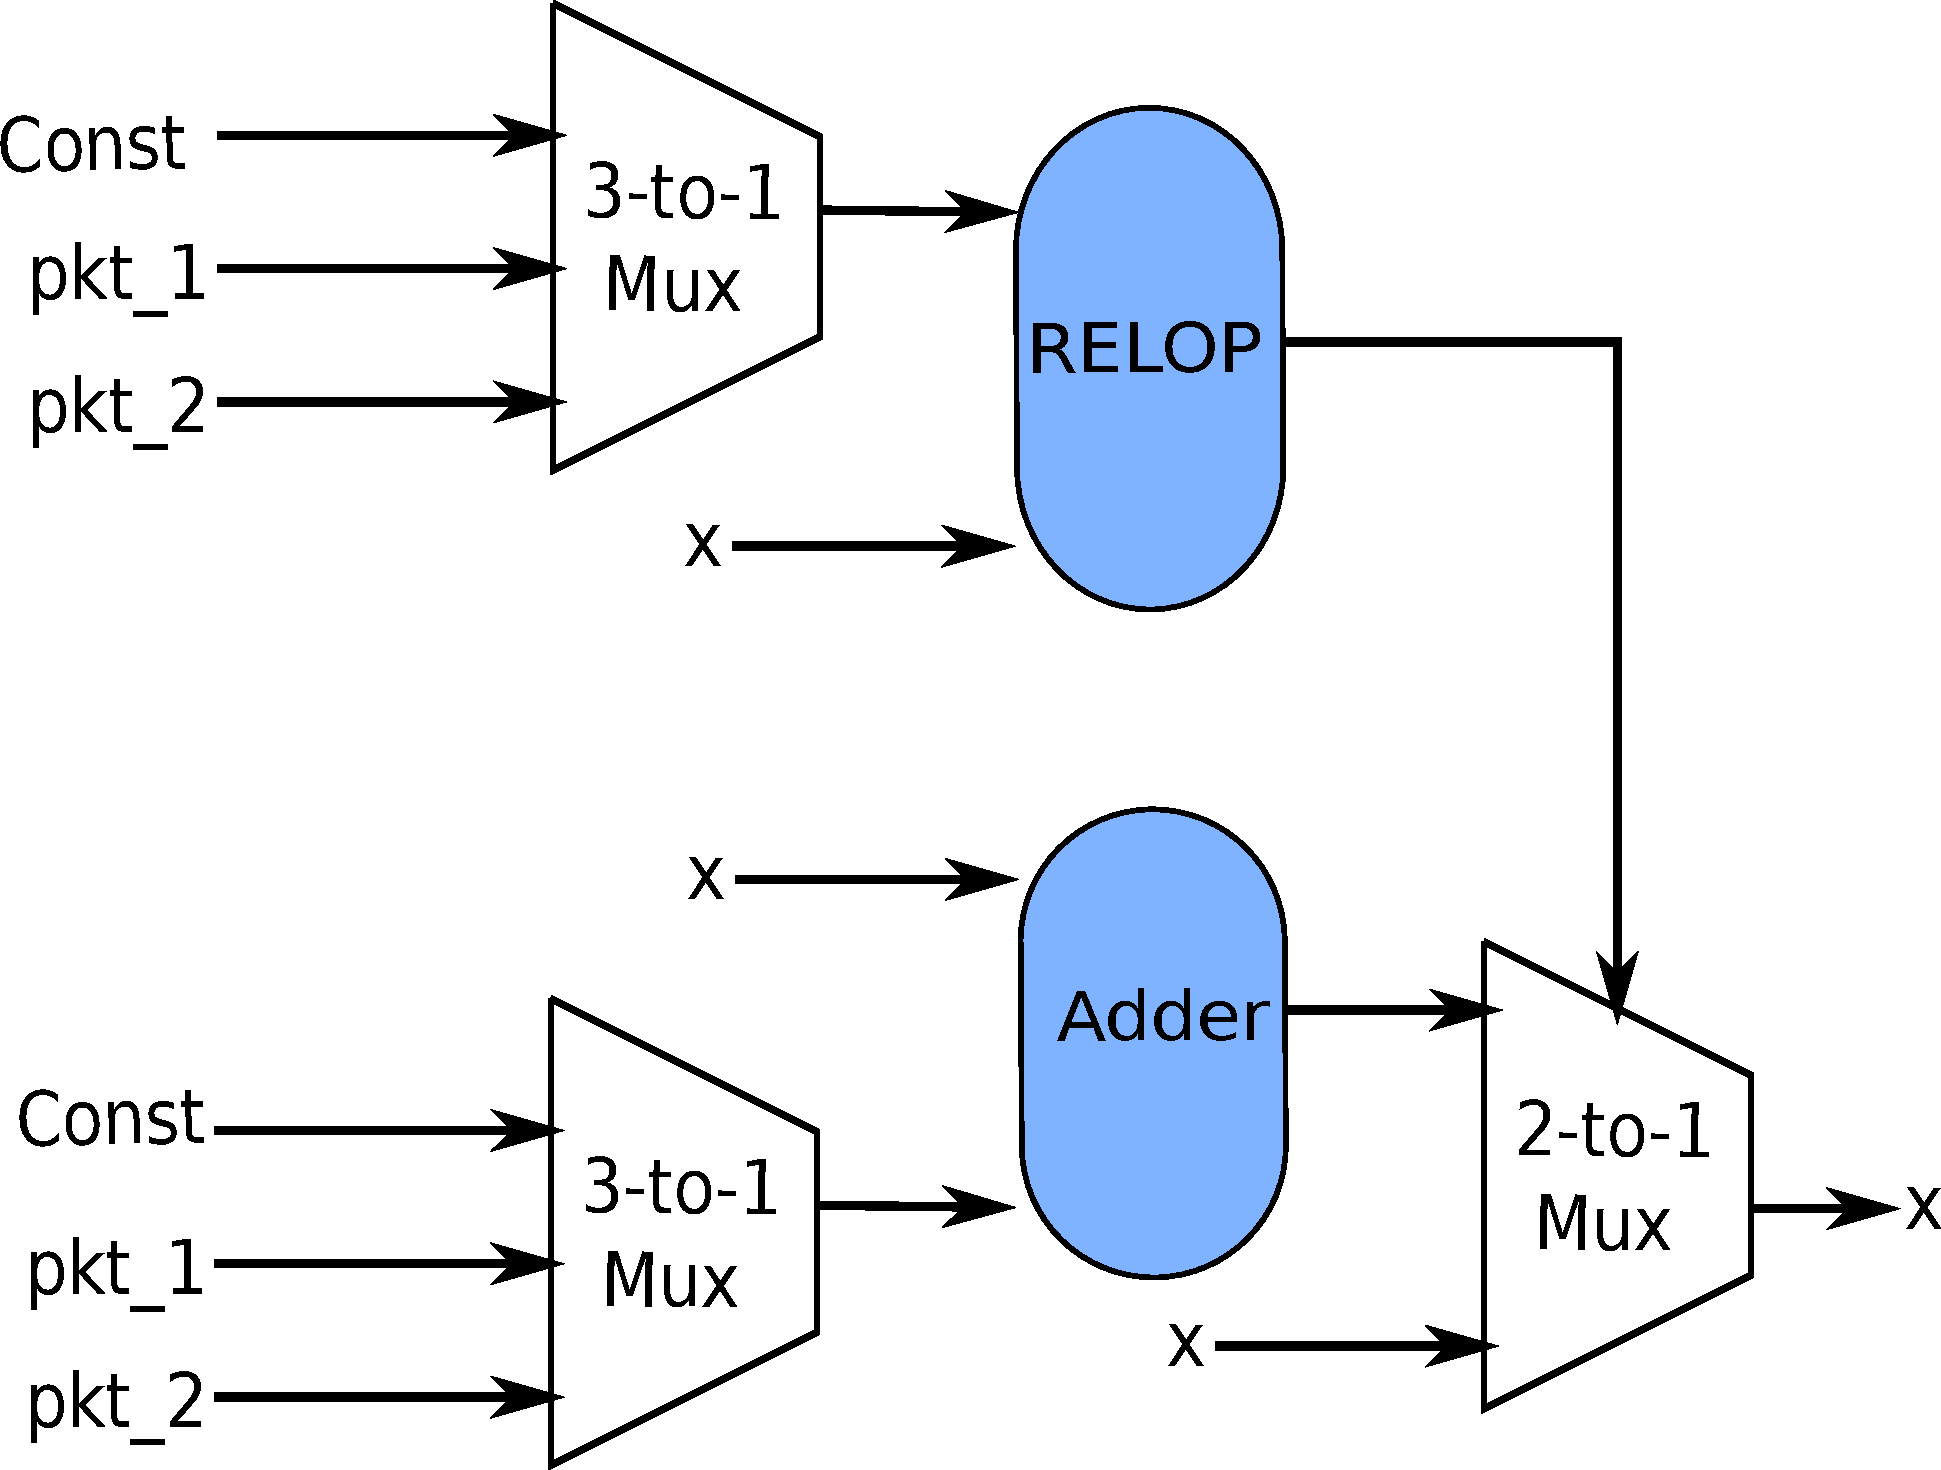
\includegraphics[width=0.3\textwidth]{pred_raw.pdf}  & 3\\
  \hline
  \end{tabular}
\end{scriptsize}
\caption{Circuit depth and propagation delay increases with complexity of atoms.}
  \label{fig:circuit_depth}
\end{table}

\begin{table*}[!t]
  \begin{tabular}{|p{0.16\textwidth}|p{0.47\textwidth}|p{0.10\textwidth}|p{0.07\textwidth}|p{0.07\textwidth}|}
\hline
Algorithm & Stateful computation & Least expressive atom & Pipeline depth & Pipeline width \\
\hline
Bloom filter~\cite{bloom} & \pbox{0.54\textwidth}{Set membership bit on every packet.} & Write & 4 & 3\\
\hline
Heavy Hitters~\cite{opensketch} & Increment Count-Min Sketch~\cite{cormode} on every packet. & RAW & 10 & 9 \\
\hline
Flowlets~\cite{flowlets} & Update saved next hop if flowlet threshold is exceeded. & PRAW & 6 & 2 \\
\hline
RCP~\cite{rcp} & \pbox{0.54\textwidth}{Accumulate RTT sum if\\RTT is under maximum allowable RTT.} & PRAW & 3 & 3 \\
\hline
Sampling & \pbox{0.54\textwidth}{Sample/Mark a packet if packet count reaches N;\\Reset count to 0 when it reaches N.} & If-Else RAW & 4 & 2\\
\hline
HULL~\cite{hull} & Update counter for virtual queue. & Sub & 7 & 1 \\
\hline
AVQ~\cite{avq} & Update virtual queue size and virtual capacity & Nested & 7 & 3 \\
\hline
CONGA~\cite{conga} & \pbox{0.54\textwidth}{Update best path's utilization/id if we see a better path.\\
                                           Update best path utilization alone if it changes.}  & Pairs & 4 & 2\\
\hline
trTCM~\cite{trTCM} & Update token counts for each token bucket & Doesn't map & 7 & 3 \\
\hline
CoDel~\cite{codel} & \pbox{0.54\textwidth}{Update:\\Whether we are dropping or not.\\Time for next drop.\\Number of drops so far.\\Time at which min. queuing delay has exceeded target.}& Doesn't map & 14 & 3\\
\hline
\end{tabular}
\caption{Data-plane algorithms}
\label{tab:algos}
\end{table*}

To evaluate \pktlanguage, we express several data-plane algorithms
(Table~\ref{tab:algos}) using \pktlanguage and determine if they are
implementable on different \absmachine machines that provide different stateful
atoms (Table~\ref{tab:templates}). Appendix A contains circuit diagrams and
SKETCH code for these atoms.

\subsection{Experimental procedure}
As mentioned in \S\ref{ss:code_gen}, we consider only stateful atoms by
assuming stateless codelets map one-to-one to stateless atoms for all
\absmachine machines. For simplicity, the stateful atoms only permit updates to
state variables and forbid packet field updates mixed in with these state
updates.  Assuming the \absmachine machine provides an atom to read a state
variable\footnote{The inability to read a state variable renders it
powerless!}, such packet updates can be treated as stateless operations in
subsequent pipeline stages.

We also assume every \absmachine machine provides exactly one stateful atom.
Table~\ref{tab:templates} gradually increases the capability of this single
atom.  We designed the atoms in Table~\ref{tab:templates}, and hence the
\absmachine machines providing them, to form a containment hierarchy: each atom
can express all data-plane algorithms that its predecessor can.

We now consider every atom/\absmachine machine from Table~\ref{tab:templates},
and every data-plane algorithm from Table~\ref{tab:algos} to determine if each
algorithm is \textit{implementable} on a particular \absmachine machine. We say
an algorithm is implementable on a \absmachine machine, if every stateful
codelet within the data-plane algorithm can be mapped (\S\ref{ss:code_gen}) to
the single stateful atom provided by the \absmachine machine. Because atoms are
arranged in a containment hierarchy, we list the \textit{least expressive} atom
that can be used to implement a data-plane algorithm in Table~\ref{tab:algos}.

\subsection{Interpreting the results}
Table~\ref{tab:algos} tells a network programmer the minimal atom required for
a data-plane algorithm to run at line rate. For an ASIC engineer designing
programmable switches, the same table describes the algorithms that are
implementable on a particular \absmachine machine with a specific stateful
atom. For instance, a \absmachine machine with the paired updates atom can
implement eight algorithms, while a machine with a simpler read-add-write atom
can implement only two.

We also discuss broader lessons for designing programmable switching chips.
First, atoms that support stateful operations only on a single state variable
are already good enough for several data-plane algorithms (Bloom Filters
through AVQ in Table~\ref{tab:algos}). However, there are data-plane algorithms
for which the switch needs to provide an ability to update a pair of state
variables based on the other's previous values. The simplest example
is CONGA, whose code we reproduce below:
\begin{verbatim}
  if (p.util < best_path_util[p.src]) {
    best_path_util[p.src] = p.util;
    best_path[p.src] = p.path_id;
  } else if (p.path_id == best_path[p.src]) {
    best_path_util[p.src] = p.util;
  }
\end{verbatim}
Here, \texttt{best\_path} (the ID of the best path for a particular
destination) is updated conditioned on \texttt{best\_path\_util} (the utilization of
the best path to that destination) and vice versa. There is no way to separate
the two state variables into separate stages and guarantee correctness.

However, even the paired update atom, where the update to a state variable is
conditioned on a predicate of a pair of variables, is insufficient.  There are
algorithms that can still not run at line-rate such as CoDel~\cite{codel} and
the two-rate three-color meter~\cite{trTCM}. The good news, however, is that
the codelets in these cases are still restricted to a pair of state variables.
We haven't yet encountered a case where a triplet of state variables all fall
in the same strongly connected component, requiring a three-way state update.
We leave the problem of approximating CoDel/trTCM to fit within a particular
atom or conversely, designing more complex atoms to support them to future work.

While a more expressive atom is strictly better for mapping data-plane
algorithms, it does have a cost. A larger atom takes up more gate area when
synthesized to a digital circuit and results in longer propagation delays. As
an illustration, consider the circuits for three atoms shown in
Figure~\ref{fig:circuit_depth}, the first three atoms from
Table~\ref{tab:templates}. We use the number of elements that a wire has to
pass through between input and output (the circuit depth) as a proxy for
propagation delay. We see that the circuit depth increases as we add
complexity to atoms. At some point, the propagation delay may be large enough
that the resulting circuit may not meet timing for a particular line rate. We
plan to synthesize these atoms to circuits in a standard cell library to study
this further.

These results will change as programmable switches evolve and network
programmers push chip boundaries with new algorithms.  The larger takeaway is
that we can now begin to quantify the programmability-performance tradeoff that
chip designers have so far had only a gut instinct for. Using the \pktlanguage
compiler, we can rigorously\footnote{Modulo inefficiencies in the compiler
itself.} determine if a particular set of high-level algorithms can run at a
given line rate, given the atoms supported by the \absmachine machine at that
line rate.

%TODO: This isn't written as strongly as we could write this.
% Not sure whether we want to have this at all.
\subsection{Compilation times}
The data-plane algorithms that we consider are all under 100 LOC. Hence, our
front-end compilation times are negligible; compilation times are dominated by
SKETCH trying to map codelets to atoms. However, we limit the bit-width of
SKETCH holes to 5 bits because the constants we see in our algorithms are
small.  This reduces the search space for SKETCH.  The worst-case occurs when a
large algorithm does not map to a large atom, because then SKETCH has to rule
out every possible configuration. Even so, our worst-case compilation time is
10 seconds when CoDel doesn't map to a \absmachine machine with the pairs atom.
This time will increase as we increase the bit width of constants that SKETCH
has to search; howerver, because the data-plane algorithms are themselves
small, we don't anticipate compilation times being a concern.
